\documentclass[tikz,border=10pt]{standalone}
% Shared look for every TikZ diagram. Load with \input{../../tools/tikz-style.tex}
\usepackage[T1]{fontenc}
\usepackage{lmodern}
\renewcommand{\sfdefault}{lmr}  % diagrams use the same serif as the text
\usetikzlibrary{arrows.meta, positioning, shapes.geometric, calc, fit, backgrounds}
\definecolor{cblue}{HTML}{4C78A8}
\definecolor{corange}{HTML}{F58518}
\definecolor{cgreen}{HTML}{54A24B}
\definecolor{cred}{HTML}{E45756}
\definecolor{cpurple}{HTML}{B279A2}
\definecolor{cgrey}{HTML}{6B6B6B}
\tikzset{
  every picture/.style={font=\sffamily, line width=1.2pt},
  box/.style={draw=#1, fill=#1!12, rounded corners=4pt, align=center, inner sep=7pt, minimum height=1.1cm},
  box/.default=cgrey,
  arrow/.style={-{Stealth[length=3mm]}, draw=cgrey, line width=1.4pt},
  title/.style={font=\sffamily\bfseries\Large},
  note/.style={font=\sffamily\small, text=cgrey, align=center},
}
\AtBeginDocument{\hyphenpenalty=10000 \exhyphenpenalty=10000}

\begin{document}
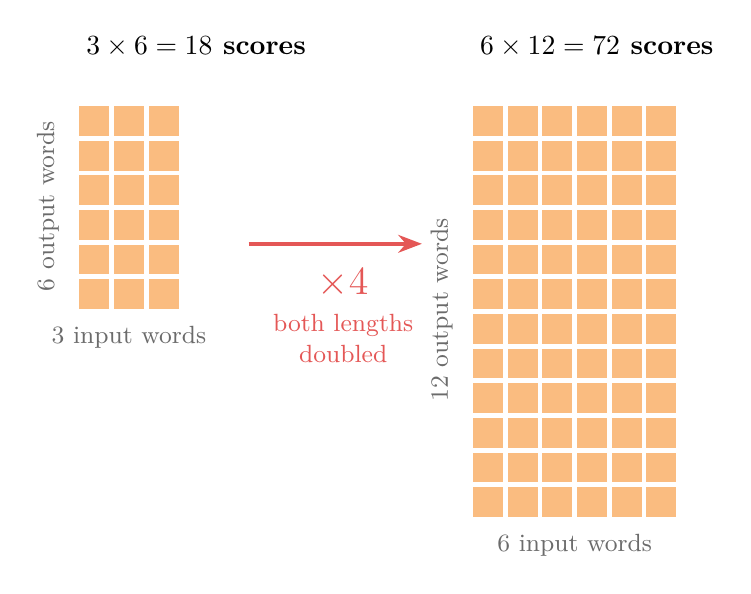
\begin{tikzpicture}[s/.style={draw=white, fill=corange!55, minimum size=0.42cm, inner sep=0pt}]
  \foreach \n/\m/\x/\lab in {3/6/0/{$3 \times 6 = 18$ scores}, 6/12/5.0/{$6 \times 12 = 72$ scores}} {
    \foreach \a in {1,...,\n} \foreach \b in {1,...,\m} \node[s] at (\x+0.44*\a,-0.44*\b) {};
    \node[font=\sffamily\bfseries, anchor=west] at (\x+0.2,0.5) {\lab};
    \node[note, rotate=90] at (\x-0.15,-0.22*\m-0.2) {\m\ output words};
    \node[note] at (\x+0.22*\n+0.22,-0.44*\m-0.55) {\n\ input words};
  }
  \node[font=\sffamily\Large, text=cred] at (3.6,-2.5) {$\times 4$};
  \draw[arrow, draw=cred] (2.4,-2.0) -- (4.6,-2.0);
  \node[note, text=cred] at (3.6,-3.2) {both lengths\\doubled};
\end{tikzpicture}
\end{document}
